\begin{figure}[ht] \centering
    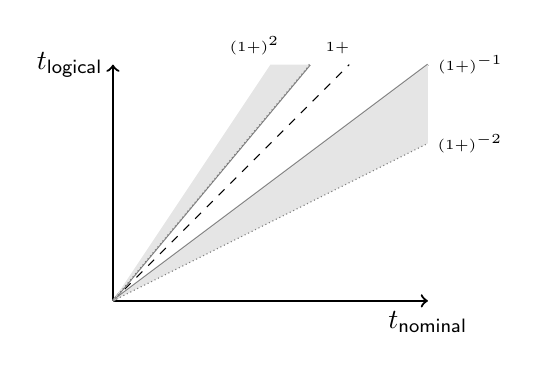
\begin{tikzpicture}
        \draw[->, thick] (0, 0) -- (4, 0) node[below] {$t_{\mathsf{nominal}}$};
        \draw[->, thick] (0, 0) -- (0, 3) node[left] {$t_{\mathsf{logical}}$};
        \draw[dashed] (0, 0) -- (3, 3);

        \draw[thick, color = gray] (0, 0) -- (4, 3) node[right, color = black] {\tiny $(1 + \clockDrift)^{-1}$};

        \draw[thick, color = gray] (0, 0) -- (2.5, 3) node[above, color = black, xshift = 1em] {\tiny $1 + \clockDrift$};

        \fill[fill = gray!20] (0, 0) -- (4, 3) -- (4, 2);
        \fill[fill = gray!20] (0, 0) -- (2, 3) -- (2.5, 3);

        \draw[densely dotted, color = gray] (0, 0)--(4, 2) node[right, color = black] {\tiny $(1 + \clockDrift)^{-2}$};
        \draw[densely dotted, color = gray] (0, 0)--(2.5, 3) node[above, color = black, xshift = -2em] {\tiny $(1 + \clockDrift)^2$};
    \end{tikzpicture}
    \caption{\sl An illustration of the logical time linear envelope (in gray) such that honest majority is necessary.}
    \label{fig:honest-majority}
\end{figure}
